\subsection{Empfehlung}

\subsubsection{Optimierungen}

\textbf{Antriebskonzept der Vereinzelung}
\newline
Der Funktionstest der Vereinzelung zeigte, dass die Zuverlässigkeit der Vereinzelung durch das Getriebespiel des Antriebs stark beeinträchtigt wird. Das Auftretten des Fehlers ist anhand von zwei Punkte erklärbar:
\begin{itemize}
	\item Das Funktionsmuster wurde ohne Motor realisiert. Durch das manuelle Testen von Hand, war Spiel eine inexistente Grösse.
	
	\item Das Ausmass des Spiels wurde während der Umsetzungsphase klar unterschätzt. Die hohe Übersetzung des Getriebemotors führt zu einem feststellbaren Spiel auf der Ausgangswelle.
\end{itemize}

Zur Eliminierung des Spiels und somit direkten Steigerung der Zuverlässigkeit werden folgende Massnahmen empfohlen:

\begin{itemize}
	\item Der qualitativ durchschnittliche Antrieb (Pololu XY) durch einen qualitativ besseren Motor ersetzen, welcher ein geringeres Spiel aufweist.
	
	\item Die Anordnung des Antriebs neu konzipieren. Dabei kann das Spiel massiv reduziert werden, indem der Antrieb an der Aussenkontur der Lochmaske gekoppelt wird. Dabei muss an der Aussenkontur eine Verzahnung realisiert werden, sodass über ein zweites Zahnrad der Motor die Rotation umsetzen kann (siehe Abbildung \ref{fig:optimierung_lochmaske}). Die Grössenordnung dieser Übersetzung ist variabel, führt jedoch bei optimaler Auslegung dazu, dass ein Antrieb mit geringerer Übersetzung verwendet werden kann. Dadurch wird das Spiel reduziert. 
\end{itemize}

\begin{figure}[H]
	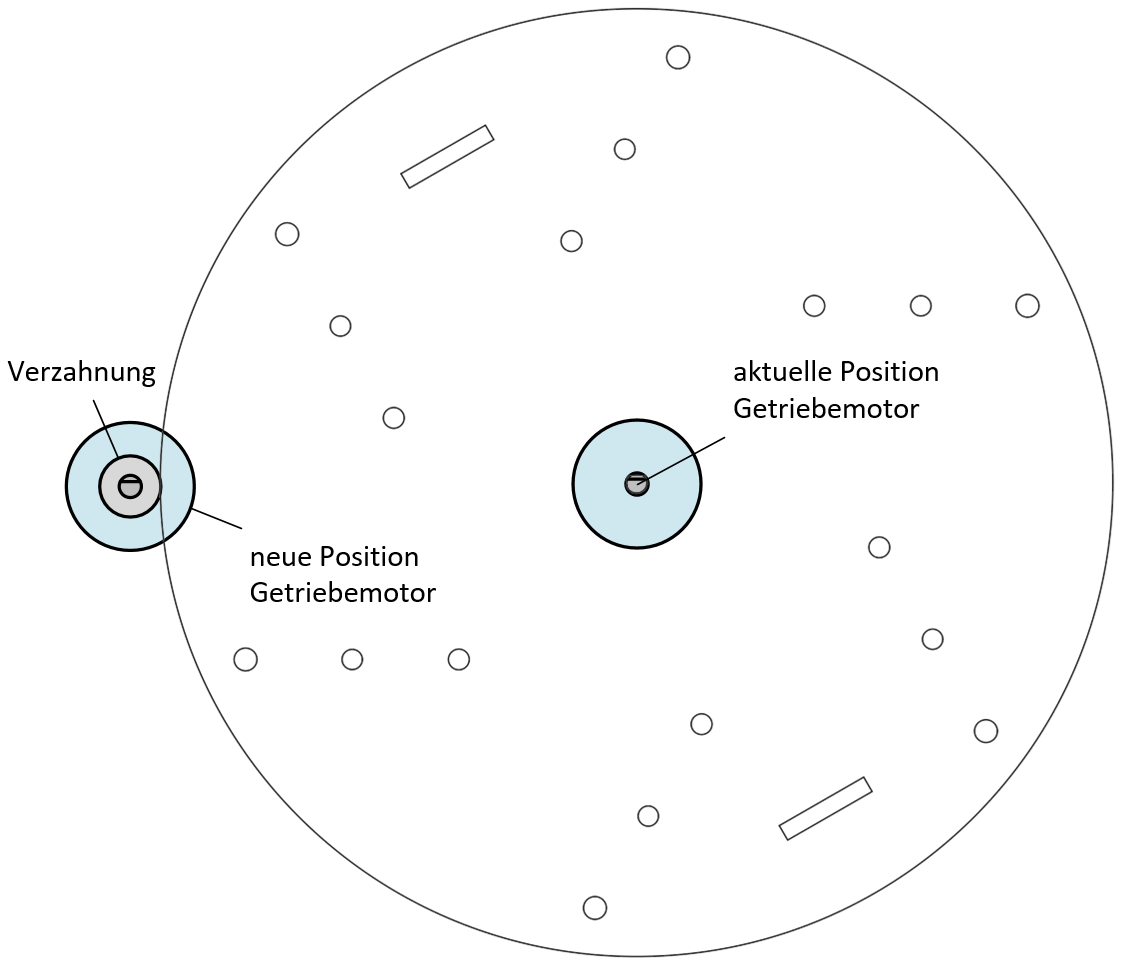
\includegraphics[scale=0.5]{Illustrationen/8-Fazit/optimierung_lochmaske.png}
	\caption{verbesserte Anordnung des Antriebs für die Lochmaske}
	\label{fig:optimierung_lochmaske}
\end{figure}